
\section{Theory of Heavy-Tailed Self Regularization}
\label{sxn:theory}


Let us write the Energy Landscape (or optimization function) for a typical DNN with $L$ layers, with activation functions $h_{l}(\cdot)$, and with $N\times M$)  weight matrices $\mathbf{W}_{l}$, and the biases $\mathbf{b}_{l}$, as follows:
\begin{equation}
E_{DNN}=h_{L}(\mathbf{W}_{L}\times h_{L-1}(\mathbf{W}_{L-1}\times h_{L-2}(\cdots)+\mathbf{b}_{L-1})+\mathbf{b}_{L})  .
\label{eqn:dnn_energy}
\end{equation}
%WLOG,
The model would be trained on some labeled data $\{d_{i},y_{i}\}\in\mathcal{D}$, using Backprop, by minimizing the loss $\mathcal{L}$
For simplicity, we do not indicate the structural details of the layers (e.g., Dense or not, Convolutions or not, Residual/Skip Connections, etc.). 
Each layer is defined by one or more layer 2D weight matrices $\mathbf{W}_{L}$, and/or the 2D feature maps $\mathbf{W}_{i,L}$ 
extracted from 2D Convolutional layers.

\charles{
In this study, we only need to consider Linear and 2D Convolutional (Conv2D) layers because we will only examine series of commonly
available, open source, pre-trained DNNs with these kinds of layers.  We describe these pre-trained models in detail below;
briefly examine the VGG series (VGG11, VGG13, VGG1, VGG19), with and without BatchNorm, the complete set of
available ResNet models ranging from ResNet10 to ResNet152(b), and a wide range of other models.  All models have
been trained on ImageNet, and reported test accuracies are available.  For our analysis, we do not needs to retrain these
models, and we do not even need access to the test data.  }


\paragraph{Random matrix models.} 

\charlesX{
We apply our new Theory of Heavy-Tailed Self Regularization (HT-SR) to analyze these large, pretrained DNNs.  
We model \emph{the correlations} arising in the DNN layers by forming the normalized correlation matrices $\mathbf{X}=(1/N)\mathbf{W}_{L}^{T}\mathbf{W}_{L}$ 
for each of the individual  the layer weight matrices $\mathbf{W}_{L}$ and then studying the eigenvalue density of each $\mathbf{X}$,  $\rho(\lambda)$.
The HT-SR Theory lets us characterize the densities because they almost always display heavy tailed signatures,
 and can be fit to a Power Law, $\rho(\lambda)\sim\lambda^{-\alpha}$, with exponent $\alpha$.   And , on average,
 the smaller the $\alpha$, the more Self Regularization is in the DNN.  Of course, the
  pretrained weight matrices  $\mathbf{W}_{L}$  themselves are not at all random because they have been trained 
  on very large, high quality data sets,
  and they behave quite differently from a random heavy tailed (i.e. Pareto) matrix.  And it is these differences we can exploit
  to predict trends in the generalization accuracy.}
  
First, some notational conventions.
For each Linear layer, we get a  single, $(N\times M)$ (real valued) 2D matrix, layer weight matrix, denoted $\mathbf{W}_{L}$, for layer $L$.  
This also includes Dense or Fully Connected (FC) layers, as well as 1D Convolutional (Conv1D) layers, Attention matrices, etc.
We ignore the bias here terms in this analysis.  Let the aspect ratio be $Q=\frac{N}{M}$, with $Q\ge 1$.
For the 2-D Convolutional Conv2D) layers, we have a 4-index Tensor, of the form $(N\times M \times c\times d)$, consisting
of $c\times d$ 2D feature maps of shape $(N\times M)$.    
We  extract $n_{L}=c\times d$  2D  weight matrices $\mathbf{W}_{L,i}$, one for each feature map $i=[1,\dots,n_{L}]$ for layer $L$.
We have not yet analyzed LSTM or other complicated Layers. 
A typical modern DNN may have anywhere between 5 and 5000 2D $\mathbf{W}_{L,i}$ layer matrices.
   
We imagine the matrix elements of $\mathbf{W}$  are drawn from some probability distribution, such as a Normal $N(0,\sigma)$ distribution
$$
Pr(W_{i,j})\sim N(0,\sigma)
$$
with zero mean and variance $\sigma$.   \charlesX{Our imagination here lets us derive seemingly \emph{Universal} expressions for how the correlations should behave, 
even though $\mathbf{W}$  itself is not at all random. }
These Gaussian models arise in the well known Marchenko-Pastur (MP) Random Matrix Theory (RMT), as well as the Spiked-Covariance model. 
Gaussian model are useful for understanding older, smallish Neural Networks, such as LeNet5.
But more modern DNNs display more exotic Universal behavior.  


\paragraph{Heavy-Tailed Universality.} 
Recent work by Martin and Mahoney~\cite{MM18_TR} 
has demonstrated that all large, modern DNNs show statistically significant, and Universal, Heavy-Tailed signatures.  
To understand this this, we use a Heavy-Tailed variant of the MP RMT, \nred{HT-RMT}.
Let 
$$
Pr(W_{i,j})\sim\dfrac{W_{0}^{\mu}}{|W_{i,j}|^{1+\mu}}  ,
$$
where $W_{0}$ is the typical order of magnitude of $W_{i,j}$, and $\mu>0$. 
The Heavy-Tailed matrix models were first introduced in the theoretical physics literature, where they are called \'L\'evy Matrices when $0<\mu<2$~\cite{PB94}.
More generally, there are at least 3 different Universality classes of Heavy-Tailed random matrices, defined by the range $\mu$ takes on:
\begin{itemize}
\item $0<\mu<2$: VHT:  Very Heavy-Tailed (sometimes called L\'evy) matrices
\item $2<\mu<4$: FT:  Fat-Tailed (or Moderately Heavy Tailed) matrices
\item $\mu>4$: WHT:  Weakly Heavy-Tailed matrices
\end{itemize}
Results for $\mu=2$ and $\mu=4$ are slightly different~\cite{SornetteBook,BouchaudPotters03}, but we don't describe them since we don't expect to be able to resolve the difference numerically.

We can identify these different Universality classes by analyzing the eigenvalue spectrum of the associated correlation matrices. 
For any layer weight matrix $\mathbf{W}$, we construct the associated $M\times M$ (uncentered) correlation matrix. 
Dropping the $l,i$ indices, we have
\begin{equation}
\mathbf{X} = \dfrac{1}{N^{\gamma}}\mathbf{W}^{T}\mathbf{W}  ,
\label{eqn:unc_corr_mat}
\end{equation}
where we normalize by $1/N^{\gamma}$. 
For our empirical analysis, $\gamma=1$. 
In theoretical treatments, $\gamma$ depends on the form of $Pr(W_{i,j})$, in order to prove the existence of the limiting forms of the ESD.
For the MP theory and Gaussian Universality class, we can set $\gamma=1$, but for the Heavy tailed Universality class, we would need to set $\gamma=2/\mu$.
Of course, in any empirical study, we do not know t the power law exponent $\mu$, or the Universality class,r \emph{a priori}, and this will be very important below. 

We now form $\mathbf{X}= \dfrac{1}{N}\mathbf{W}^{T}\mathbf{W}$, normalized using $\gamma=1$, and compute the eigenvalue spectrum of $\mathbf{X}$, 
$$
\mathbf{X}\mathbf{v}_{i}=\lambda_{i}\mathbf{v}_{i}
$$

We call the density of eigenvalues $\rho(\lambda)$ the Empirical Spectral Density (ESD).  This is just a histogram of the eigenvalues, formally written as

$$\rho(\lambda)=\sum\limits_{i=1}^{M}\delta(\lambda-\lambda_{i})$$

The heavy tailed RMT theory tells us that ESD  $\rho(\lambda)$ of any heavy tailed matrix will have a heavy tail, and take the form
$$
\rho(\lambda)\sim\lambda^{-\alpha}
$$
which is (at least) valid within a bounded range of eigenvalues $\lambda\in[\lambda_{min},\lambda_{max}]$.  
\charles{Discuss fact the power law tails are Frechet at finite size so only need to fit the bulk}

We then fit the bulk of the ESD to a power law using the commonly accepted Maximum Likelihood (MLE) method of Clauset et. al..
This method works very well for exponents in the  Fat Tailed Universality class, where $\alpha\in[2,4]$,
and is sufficient, although imprecise for smaller and larger $\alpha$.  The fitting method is robust in that it is  reasonably
insensitive to the the choice of normalization $\gamma=1$.

\charles{Moved paragraphs around a bit here}

In modern, pre-trained DNN, we find that the ESD of nearly every \ $\mathbf{W}$ layer matrix can be fit to a power law,
%The layer matrices in all large, modern DNNs, do not have a scale cut-off, and, instead display scale-invariance.  
We have examined nearly 10,000 layer weight matrices $\mathbf{W}_{l,i}$ across over 50 different modern. pre-trained DNN architectures.  
 $70-80\%$ of the time, the power law exponent lies in the range of the Fat Tailed Universality class.
And for $10-20\%$ of the time, the ESDs display Very Heavy-Tailed signatures.
Of course, there are exceptions, and in any real DNN,  $\alpha$ may range anywhere from $\sim1.5$ to $10$ or higher.  

This kind of Universality of exponents is very special in theoretical physics and indicates the presence of a deeper, 
underlying mechanism driving the system.  Indeed, it is this Universality that has motivated this study.

\michael{can you please add numbers to these equations:  I use them  in the derivation}

For the VHT Universality class, this power law tail persists in the infinite limit $N\rightarrow\infty$, $Q$ fixed.
And we have the linear relation between our observed exponent $\alpha$ and the theoretical $\mu$

$$\alpha=\dfrac{1}{2}\mu+1$$

which works very well even for very small matrices $(M\sim100)$.
For the FHT Universality class, $\alpha$ is still linear in $\mu$, but displays very strong finite size effects, giving $\alpha=a+b\mu$, where $a,b$ depend strongly on $M,N$. Also,  the power law tail vanishes in the limit, but persists at all finite sizes, and follows a Frechet distribution (i.e. an exponentially truncated power law). \nred{In both cases, we expect the maximum empirical eigenvalue $\lambda_{max}$ will scale with N (with Q=1) according to Extreme Value Theory (EVT)~\cite{MM18_TR,XXX,XXX}

$$\lambda_{max}\sim N^{4/\mu-1}$$

Amazingly, \emph{due to Universality,} we expect this relation to hold even when the matrix $\mathbf{W}$ is not itself heavy tailed random and therefore not governed by EVT.
}
These strong finite size effects characterize these so-called Fat Tailed distributions; they are also well known in the physics literature\cite{SornetteBook,BouchaudPotters03}. 
And it is these finite size effects that we will exploit to develop our theory.


\paragraph{A Universal DNN Complexity Metric.} 

The power law exponent $\alpha$ is a complexity metric for a weight matrix; it describes how well that matrix encodes the complex correlations in the training data.
Thus, a natural class of complexity metrics to consider for a DNN is to take a weighted average of the power law exponents $\alpha_{l,i}$ for each layer weight matrix $\mathbf{W}_{l,i}$, given as follows:
\begin{equation}
\hat{\alpha}:=\dfrac{1}{n}\sum_{l,i}b_{l,i}\alpha_{l,i}  .
\label{eqn:alpha_hat_generic}
\end{equation}
Here, the smaller $\hat{\alpha}$, the better we expect the DNN to represent the training data, and (presumably) the better the DNN will generalize to new data.
The only question is, what are good weights $b_{l,i}$ ?

It turns out, we can extract the weighted average $\hat{\alpha}$ directly from the more familiar Product Norm, and exploiting the finite size effects of our Fat Tailed weight matrices.

%%%\paragraph{THEOREM:} \emph{The data dependent VC-like complexity of a Deep Neural Network can be expressed a weighted average the of power law exponents describing the empirical spectral density of the layer weight matrices}
%%
%%%\charles{\paragraph{PROOF:...}}

\paragraph{Product Norm Measures of Complexity.} 

Recently it has been suggested that the complexity, $\mathcal{C}$, of a DNN can be characterized by the product of the norms of the layer weight matrices,
$$
\mathcal{C}\sim\Vert\mathbf{W}_{1}\Vert\times\Vert\mathbf{W}_{2}\Vert\cdots\Vert\mathbf{W}_{L}\Vert ,
$$
where $\Vert\mathbf{W}\Vert$ may be the Frobenius norm or even the L1-norm. 
(Here we can use either $\Vert\mathbf{W}\Vert$ or $\Vert\mathbf{W}\Vert^{2}$ for our complexity metric, which will make more sense below, and one can view $\mathcal{C}$ as something akin to a data dependent VC complexity.)

To that end, we consider a log complexity
\begin{eqnarray*}
\log\mathcal{C} &\sim& \log\bigg[\Vert\mathbf{W}_{1}\Vert\times\Vert\mathbf{W}_{2}\Vert\cdots\Vert\mathbf{W}_{L}\Vert\bigg]  \\
                &\sim& \bigg[\log\Vert\mathbf{W}_{1}\Vert+\log\Vert\mathbf{W}_{2}\Vert\cdots\log\Vert\mathbf{W}_{L}\Vert\bigg]  ,
\end{eqnarray*}
and we define the average log norm of the weight matrices as
$$
\langle\log\Vert\mathbf{W}\Vert\rangle=\dfrac{1}{N_{L}}\sum_{L}\log\Vert\mathbf{W}_{L}\Vert  .
$$
(As illustrated in Figure~\ref{fig:vgg_lognorms}, this metric is a relatively good complexity metric for comparing the test accuracies of different, pre-trained DNNs in the same series.)


\paragraph{Relation to Heavy-Tailed Universality.} 

We would like to relate the empirical Frobenius norm $\Vert\mathbf{W}\Vert_{F}$ to the empirical power law exponent $\alpha$, 
and we would like this for all \nred{Heavy Tailed} Universality classes, and for the strongly correlated,  non-random, finite size empirical DNN 
layer weight matrices.  

%{To do this, we rely upon the known theoretical results for Heavy tailed random matrices, but we also need to be careful about the normalization we use.}

More-so, to demonstrate the effectiveness of the approach, we will test these relations with numerical simulations of Heavy tailed Pareto matrices.

\charlesX{Doing so, however, requires care because the pretrained $\mathbf{W}$ are not heavy tailed random matrices, and the empirical
Frobenius norm behaves very differently from a random Pareto matrix.  Figure XXX displays the direct relation between
 the power law exponents and the Frobenius norm (squared) for both randomly generated heavy tailed matrices, and the weight matrices
(extracted from the Conv2D Feature Maps) from the pre-trained VGG11 DNN.
 
 
 \begin{figure}[!htb]
    \centering
    \subfigure[Random Pareto Matrices] {
        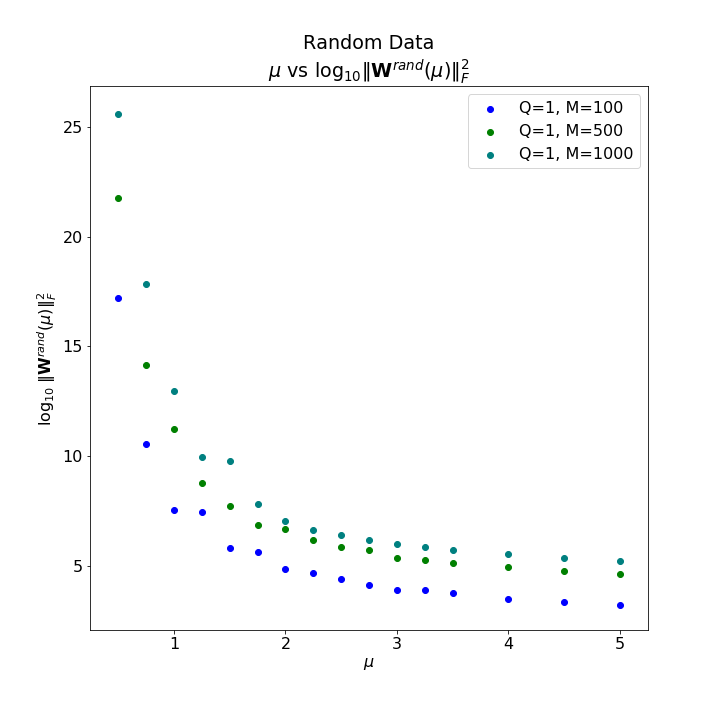
\includegraphics[scale=0.3]{img/fro-rand.png} 
        \label{fig:fro-rand}
    }
    \subfigure[VGG 11 Weight matrices]{
        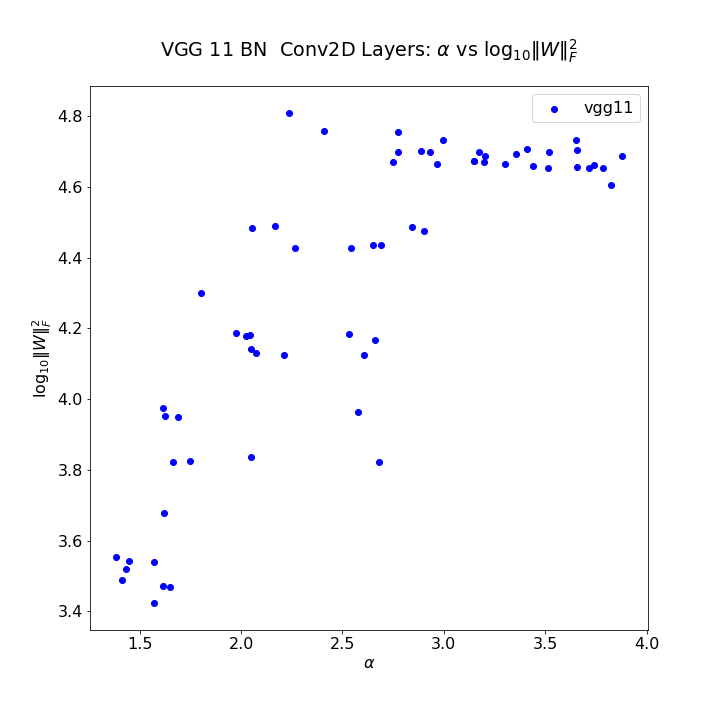
\includegraphics[scale=0.3]{img/fro-vgg11.png} 
        \label{fig:fro-vgg11}
    }
        \caption{Dependence of Frobenius Norm on Power Law exponents}
    \label{fig:fnorm}
\end{figure}



 For a random Pareto matrix $\mathbf{W}^{rand}(\mu)$,  the Frobenius norm  $\Vert\mathbf{W}^{rand}(\mu)\Vert_{F}$ increases with 
 decreasing exponent $(\mu)$;  as the tails of the ESD $\rho(\lambda)$ get heavier, the largest eigenvalue $\lambda_{max}$ of $\mathbf{X}$
  scales with the largest element of  $\mathbf{W}^{rand}(\mu)$.  But for the weight matrices of a pretrained DNN,
  the Frobenius norm $\Vert\mathbf{W}\Vert_{F}$ increases with \emph{increasing} exponent $(\alpha)$, saturating at $\alpha\approx 3$.
  This happens because the pretrained matrices  $\mathbf{W}$ themselves are highly correlated, not random matrices
  with a single large, atypical element.   And, yet, the ESD $\rho(\lambda)$ of the correlations matrices $\mathbf{X}$ display
  Universal Heavy Tailed behavior. This is one of the amazing properties of Universality.
  Of course, we expect this behavior from our  HT-SR theory; smaller exponents indicate suggest more regularization
  and therefor better generalization.  Likewise, smaller matrix norms also suggest this.  
  So to form a relation between $\alpha$ and  $\Vert\mathbf{W}\Vert_{F}$ , we will exploit Universality.  

We will derive a simple linear relation between the relation the Frobenius norm (squared) $\Vert\mathbf{W}\Vert^{2}_{F}$, the
power law exponent  $\alpha$ , and the maximum eigenvalue $\lambda_{max}$ of $\mathbf{X}$ (i.e. the Spectral Norm).  

$$\alpha\log\;\lambda_{max}\sim\log\;\Vert\mathbf{W}\Vert^{2}_{F}$$

This approximate relation formally only hold in the asymptotic limit of very small power law exponents $\alpha\rightarrow 1$ for
random heavy tailed matrices, but using Universality, we can safely extend it up to the finite size Fat-Tailed class, with
exponents $\alpha=4$ (and larger).  

We provide a simple proof below, and more details in the Appendix}.

Will also demonstrate that this relation holds numerically for both Heavy Tailed random matrices and for 
the weight matrices in pretrained DNNs.
%between the Power Law exponent and the Log Frobenius Norm numerically. 
\nred{Below}  we generate a large number of random Heavy-Tailed random matrices $\mathbf{W}^{rand}(\mu,M)$, 
with different number of eigenvalues $M$ (with aspect ratio $Q=1$), 
and drawn from a Pareto distributions with exponents $\mu\in[0.5, 5]$

$$\Pr[{W}^{rand}_{i,j}]\sim\dfrac{1}{x^{1+\mu}}$$

We fit the ESD of each $\mathbf{W}^{rand}(\mu)$ to a power law using the method of Clauset et. al. to obtain the empirical exponent $\alpha$.  

\charles{describe, give pesudocode}.

For the Universality class of VHT ($1<\mu<2$), in order to form the limiting eigenvalue distribution $\rho_{\infty}(\lambda)$,
we require that the sum of any row of $\mathbf{W}$ converges as $N\rightarrow\infty$. This means a largest  element of any row
must be of order $\mathcal{O}(1)$.  By eqn (x) above, this implies that a typical element  (i.e the variance) scales as $\mathbf{W}^{0}\sim N^{-1/\mu}$, where $1<\mu<2$.
Of course, we do not known $\mu$, and most matrices are only moderately Heavy-Tailed, not very Heavy-Tailed.
Indeed, we are using RMT to model a strongly correlated system, so the scaling parameter
we have is the power law exponent $\alpha$ from our empirical fit.
Moreover, in a practical setting, we normalize $\mathbf{X}$ by $1/N$, but the empirical variance is not $1/N$, it is determined by the Frobenius norm squared
$\Vert\mathbf{W}\Vert^{2}_{F}$.   

We note that squared Frobenius norm is just the Trace of $\mathbf{W}^{T}\mathbf{W}$
\nred{which is just the sum of the Singular Values  $\sigma_{i}$ of $M$ squared:}

$$\Vert\mathbf{W}\Vert_{F}^{2}=Tr[\mathbf{W}^{T}\mathbf{W}]=\sum_{i=1}^{M}\sigma^{2}_{i}$$

If we normalize the correlation matrix $\mathbf{X}$ by $N^{2/\mu}$, we have

$$\tilde{\mathbf{X}}=\dfrac{1}{N^{2/\mu}}\mathbf{W}^{T}\mathbf{W}$$

Call $\tilde{\lambda}$ the \emph{scale-free} eigenvalue(s) of $\tilde{\mathbf{X}}$.

$$\tilde{\mathbf{X}}\mathbf{v}=\tilde{\mathbf{X}}\tilde{\lambda}$$

If compute the scale-free eigenvalues, and fit them to a power law exponent $\tilde{\alpha}$, we find that the Frobenius norm is dominated by the maximum (scaled) eigenvalue $\tilde{\lambda}$ of $\tilde{\mathbf{X}}$.  
This is depicted in Figure 
  \ref{fig:logNormHat}
for our simulated Pareto matrices  $\mathbf{W}^{rand}(\mu)$ which shows
the log Frobenius norm squared, $\log_{10}\Vert\mathbf{W}\Vert^{2}_{F}$, divided by $\log_{10}\tilde{\lambda}$,
for all for all ranges of $\mu$

\begin{figure}[!htb]
 \centering
   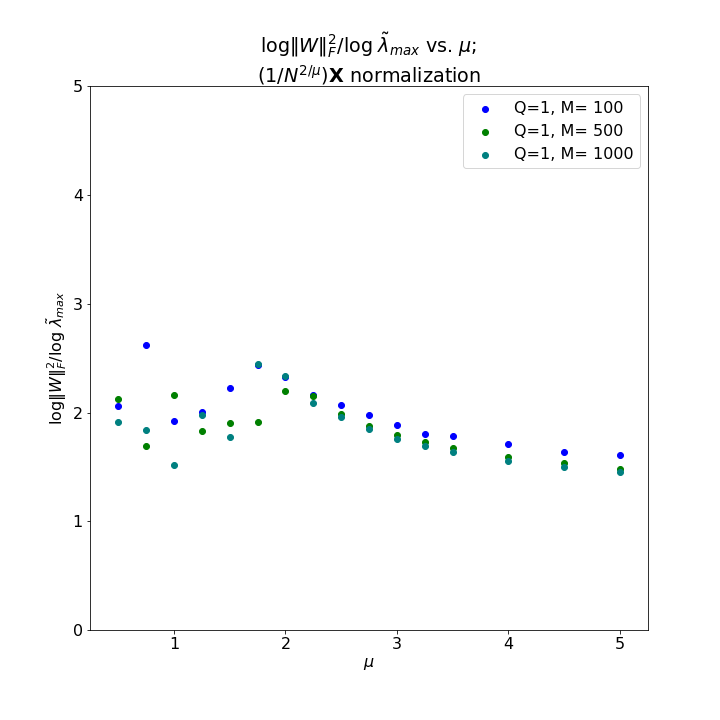
\includegraphics[scale=0.40]{img/LogNorm-Lmax-Scaled.png}
   \caption{R XXX.  WE MAY WANT THREE SUBFIGURES HERE.}
  \label{fig:logNormHat}
\end{figure}

\charlesX{UGH I forgot why this is 2 .. we need to review the data and what was done and check the math carefully}

Notice that this linear relations holds quite well, albeit with a large error bar, for $1<\mu<2$, even for small matrices, but starts to degrade for $\mu>2$.
This simple linear relation characterizes the scale invariant properties of the VHT Levy matrices; they are dominated by the largest scale-free eigenvalue.

$$\Vert\mathbf{W^{rand}(\mu)}\Vert^{2}_{F}\approx\tilde{\lambda}_{max},\;\;\mu=1$$

\nred{This might need to be
$$\Vert\mathbf{W^{rand}(\mu)}\Vert^{2}_{F}\approx\tilde{\sigma}^{2}_{max},\;\;\mu=1$$
}

which is good to within $5\%$ on a log scale

$$\log\;\Vert\mathbf{W^{rand}(\mu)}\Vert^{2}_{F}\approx\log\;\tilde{\lambda}_{max},\;\;1<\mu<2$$


If, however, we use the scale-dependent $1/N$ normalization to compute the correlations $\mathbf{X}$, we get very different behavior.
Figure~\ref{fig:randW} displays the same as above, as a function of the power law exponent \nred{(that was fit)}
$$
\dfrac{\log\Vert\mathbf{W}\Vert^{2}_{F}}{\log\lambda_{max}}\;\;vs.\;\;(\alpha)  .
$$

\begin{figure}[!htb]
 \centering
   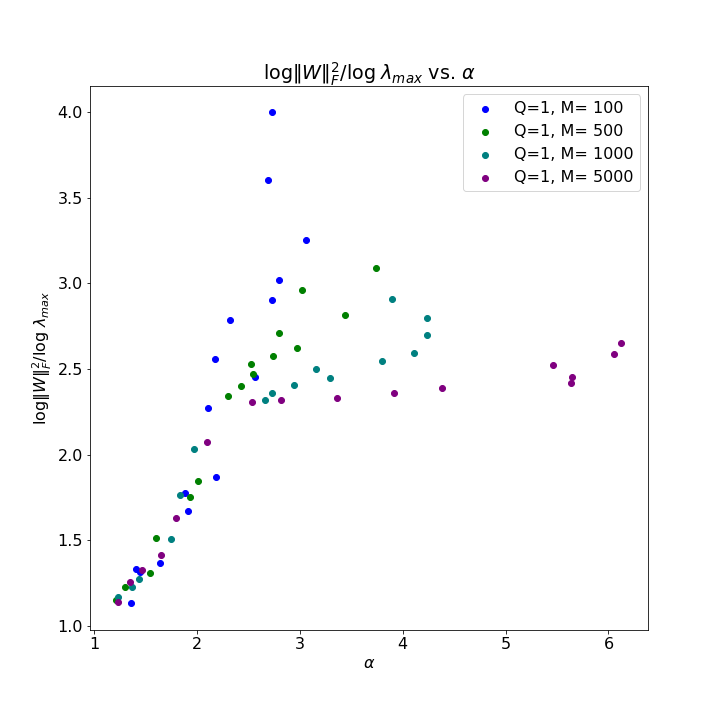
\includegraphics[scale=0.40]{img/Alpha-LogNorm-Relations.png}
   \caption{
Numerical test of the  Power Law - Norm Relation for random Heavy-Tailed matrices.
XXX.  WE MAY WANT TO PUT REAL DATA AS A SUBFIGURE HERE.
}
  \label{fig:randW}
\end{figure}

\charlesX{This is easy to derive using the our expression for $\lambda_{max}$ (above)

Let us approximate the Frobenius Norm (squared) by the maximum eigenvalue of $\mathbf{X}$

$$ \Vert W\Vert^{2}=Tr[\mathbf{W}^{T}\mathbf{W}]=N\;Tr[\mathbf{X}]\approx N\lambda_{max}$$

which is pretty good for very small $\mu$ because $\lambda_{max}$ is extremely large
when the tail is very, very long.  (This can made more rigorous, maybe in the Appendix).

Take the log of both sides and expand

$$ \log\Vert W\Vert^{2}\approx log[N\lambda_{max}]$$

$$ 2\log\Vert W\Vert\approx log N+\log\lambda_{max}$$

With a little rearrangements we find

$$ \dfrac{2\log\Vert W\Vert}{log\lambda_{max}}\approx \dfrac{log N}{log\lambda_{max}}+1$$

$$ \alpha\approx \dfrac{log N}{log\lambda_{max}}+1$$

$$ \alpha-1\approx \dfrac{log N}{log\lambda_{max}}$$

We now apply our relation betweemn $\alpha$ and $\mu$ for the VHT Universality class

$$ \alpha=\dfrac{1}{2}\mu+1$$

$$ \alpha-1=\dfrac{1}{2}\mu$$

Inserting this gives the relation we need to prove

$$ \dfrac{log N}{log\lambda_{max}}\approx\dfrac{1}{2}\mu $$

Using now the relation for the tail statistic, we have

$$ \lambda_{max}\approx N^{4/\mu-1}$$

$$ \log\lambda_{max}\approx\log N^{4/\mu-1}=(4/\mu-1)log N$$

$$ \dfrac{log N}{log\lambda_{max}}\approx\dfrac{\log N}{(4/\mu-1)log N}=\dfrac{1}{4/\mu-1}$$

We can now form the Taylor Series for $\dfrac{1}{4/\mu-1}$ around $\mu=1.15\approx 1$, which gives 

$$\dfrac{1}{4/\mu-1}\bigg\rvert_{\mu=1.15}\approx\dfrac{1}{2}\mu-\dfrac{1}{6}+\cdots\approx\dfrac{1}{2}\mu$$

And we have now derived the approximate, and surprising, linear relation we want for $\mu >= 1$ 

This is an asymptotic relation for theVHT Universality class, but we will extend it 
into the Fat Tailed (FT) Universality class, where it applies for the finite size weight matrices in DNNs.
}

The numerical results for the the Power Law-Norm relation shows several interesting features: 
First, as $\alpha$ increases, we see the relation for
\begin{itemize}
\item  $\alpha<2$ , a near linear relation 
\item  $\alpha>2$ for $N,M$ large, the relation saturates, becoming constant
\item   $\alpha>2$  for smaller $N,M$,  a nearly linear relation, but with strong finite size effects
\end{itemize}
These observations lead to a novel linear relation between the Frobenius norm and the power law exponent for our Heavy tailed matrices:
$$
\log\Vert\mathbf{W}\Vert^{2}_{F}\approx\alpha\log\lambda_{max}  ,
$$
which works very well for VHT Levy matrices, $\alpha<2$, and is a good approximation for moderately Heavy (Fat) and even some Weakly Heavy matrices. 
And we believe this is the first time this relation has been noted in the literature.

\charlesX{Explain Log Stable Rank}

We then examine a the empirical relation between  the Log-Units Stable Rank 
$\mathcal{S}^{log}_{Rank}$ and the ESD Power Law exponent $\alpha$

\emph{Log-Units Stable Rank:  } 
$$\mathcal{S}^{log}_{Rank}:=\dfrac{\log\Vert\mathbf{W}\Vert^{2}_{F}}{\log\lambda_{max}}$$

\charlesX{I am not sure why the slope is not negative...the eigenvalues are VERY LARGE, and $\log\lambda_{max}~3-5$ so this just is OFF.
Are we missing something in the derivation, like the fact that the norm squared has to be positive ?  HELP}


\paragraph{Defining the Layer Weight Matrices.} 

\charles{Here we describe how we exact the matrices. Kinda did this above already. We have not done this yet for convolutional layers--thats \emph{another} paper}

$$\text{Linear Layer:}\;\;\log\Vert\mathbf{W}_{L}\Vert^{2}_{F}\rightarrow\log\lambda^{max}_{L}\alpha_{L}$$

For the Conv2D layers, we relate the 'Norm' of the 4-index Tensor $\mathbf{W}_{l}$ to the sum of the $n_{L}=c\times d$ terms for each feature map, giving 

$$\text{Conv2D Layer:}\;\;\log\Vert\mathbf{W}_{L}\Vert^{2}_{F}\rightarrow \sum_{i=1}^{n_{L}}\log\lambda^{max}_{i,L}\alpha_{L,i}$$

We also note that $\log\Vert\mathbf{W}_{L}\Vert^{2}_{F}=2\log\Vert\mathbf{W}_{L}\Vert_{F}$ 

So in the expression for the product norm for $\log\mathcal{C}$, we can replace each $\log\Vert\mathbf{W}_{L}\Vert$ term for layer $L$ with the corresponding above expressions, and take the average over all $N_{\alpha}$  matrices.  This lets us relate the product norm complexity metric to the weighted average of power law exponents, giving

$$2\log\mathcal{C}=\langle\log\Vert\mathbf{W}\Vert^{2}_{F}\rangle\rightarrow\hat{\alpha}$$ 

where

\begin{equation}
\hat{\alpha}:=\dfrac{1}{N_{\alpha}}\sum_{i,l}\log\lambda^{max}_{i,j}\alpha_{i,l}  .
\label{eqn:alpha_hat_specific}
\end{equation}

This expression resembles the more familiar product norm, but accounts for finite size effects that the product norm relation over estimates.
% move below?
Our approach improves on the loose bound provided by the product norm, giving a more accurate expression for predicting trends
in the average case test accuracy for real world production quality DNNs.

We can now use $\hat{\alpha}$ to analyze numerous pre-trained DNNs...and the results are indeed surprising.


